\section{Frequency mode 08}
\label{sec:fm08}

\subsection{Overview}
\label{sec:fm08:overview}
Frequency mode~08 monitors two bands, $488.950$--$489.350\,\mathrm{GHz}$ and
$488.350$--$488.750\,\mathrm{GHz}$. Its main use is retrievals of \chem{O_3}
and \chem{H_2O}.

\TODO{General text about FM08}
\TODO{Show spectra?}

\subsection{Comparison of retrieved profiles}
\label{sec:fm08:comparison}


%%%%%%
% O3 %
%%%%%%

\subsubsection{\chem{O_3}}
\label{sec:fm08:comparison:O3}
The retrievals for \chem{O_3} have been compared with data from the MIPAS, MLS,
OSIRIS and SAGE~III instruments. Annual average differences to these
instruments are shown in Figure~\ref{fig:fm08:O3:profiles}. In
Figure~\ref{fig:fm08:O3:scatter} individual retrievals for the instruments for
the entire period are plotted against the retrievals from the new and old
versions of the \smr\ processing chain. The results show a considerable
improvement with the updated version of the processing compared to all
considered instruments. The over-all correlation is much better, though a
systematic under estimation remains.
\TODO{reference Fig.~\ref{fig:fm08:O3:mr_avk} in text!}

\begin{figure}[htpb]
    \centering
    \begin{subfigure}[b]{0.49\textwidth}
        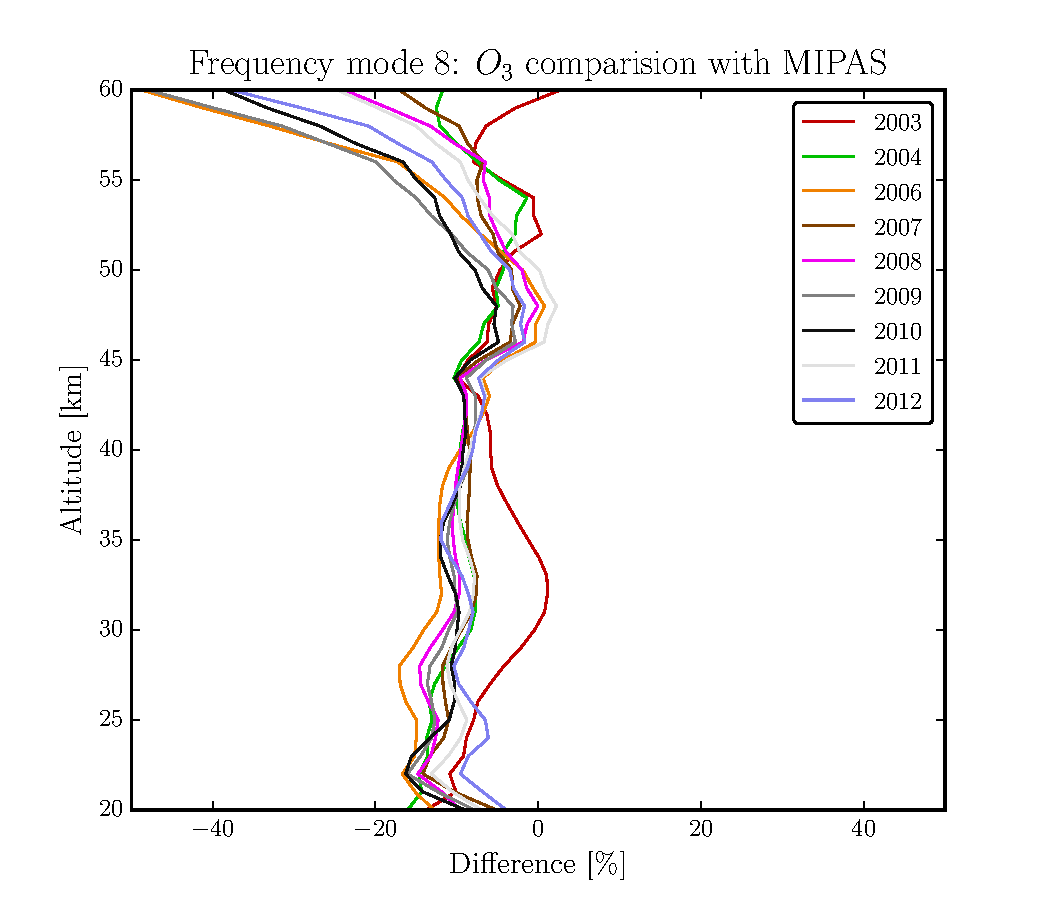
\includegraphics[width=\textwidth]{DDS_fm8_O3_perdiff_mipas}
        \caption{average difference to MIPAS}
        \label{fig:fm08:O3:profiles:MIPAS}
    \end{subfigure}
    \,
    \begin{subfigure}[b]{0.49\textwidth}
        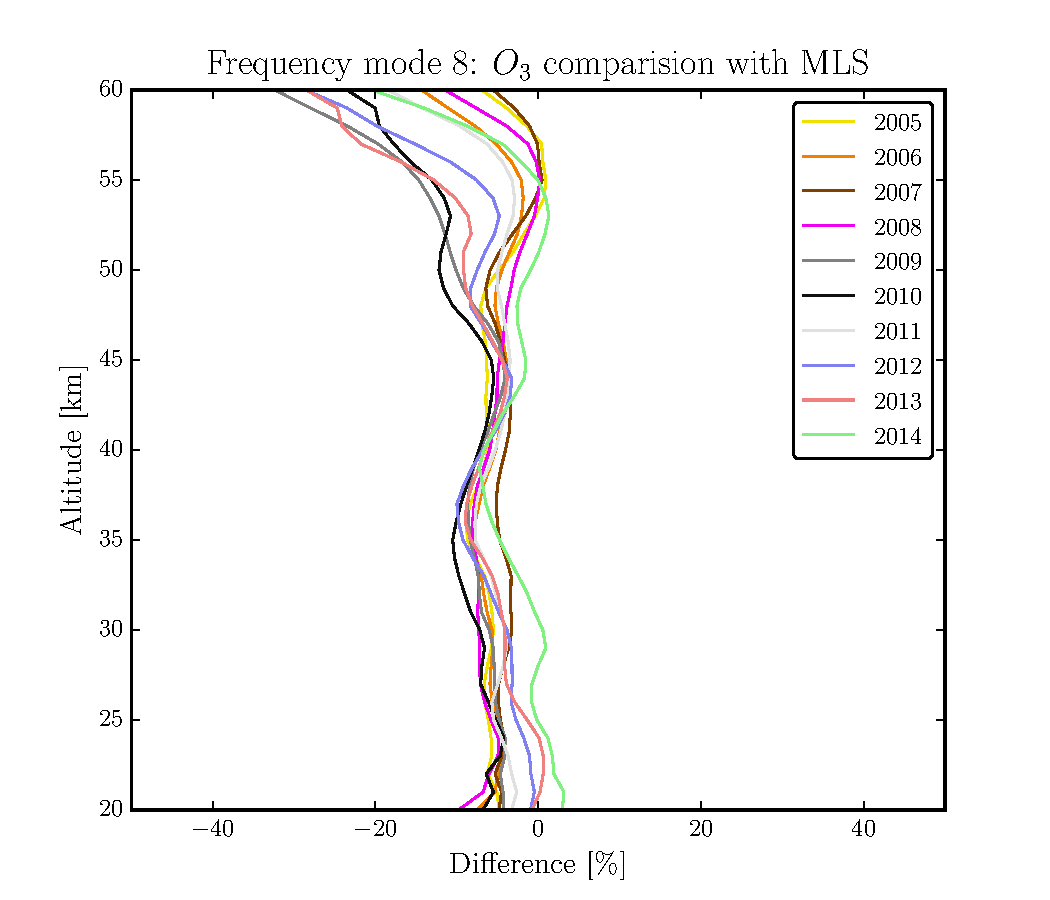
\includegraphics[width=\textwidth]{DDS_fm8_O3_perdiff_mls}
        \caption{average difference to MLS}
        \label{fig:fm08:O3:profiles:MLS}
    \end{subfigure}

    \begin{subfigure}[b]{0.49\textwidth}
        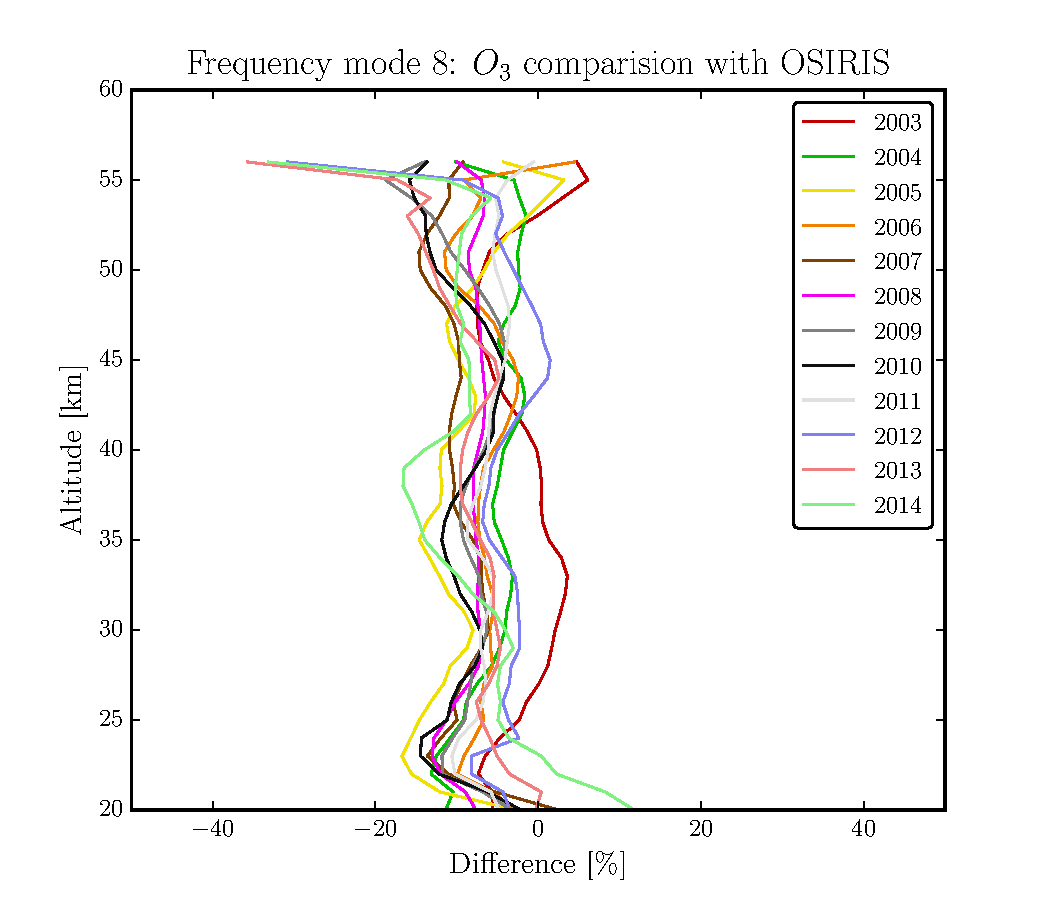
\includegraphics[width=\textwidth]{DDS_fm8_O3_perdiff_osiris}
        \caption{average difference to OSIRIS}
        \label{fig:fm08:O3:profiles:OSIRIS}
    \end{subfigure}
    \,
    \begin{subfigure}[b]{0.49\textwidth}
        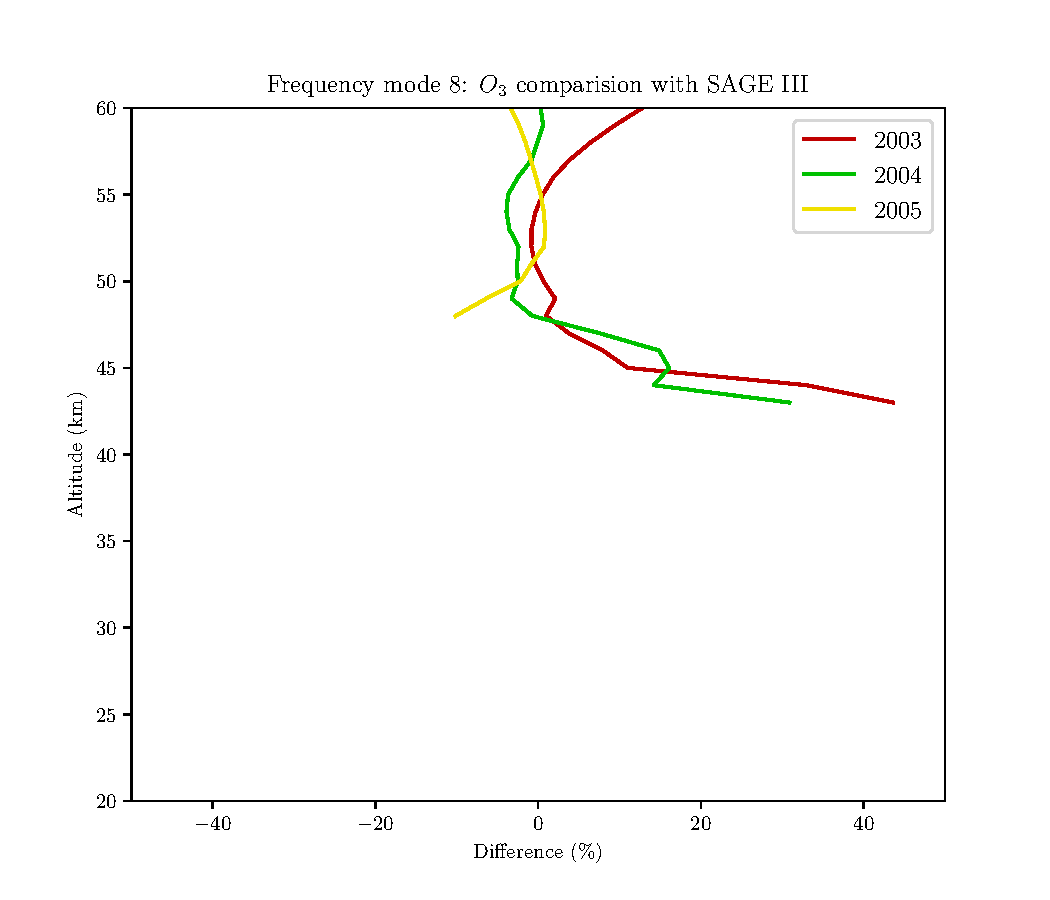
\includegraphics[width=\textwidth]{DDS_fm8_O3_perdiff_sage}
        \caption{average difference to SAGE~III}
        \label{fig:fm08:O3:profiles:SAGEIII}
    \end{subfigure}
    \caption{Average difference in percent between retrievals of \chem{O_3}
    from \smr~v3 and collocated measurements from various instruments at
    different altitudes for frequency mode~08.}

    \label{fig:fm08:O3:profiles}
\end{figure}

\begin{figure}[htpb]
    \centering
    \begin{subfigure}[b]{0.49\textwidth}
        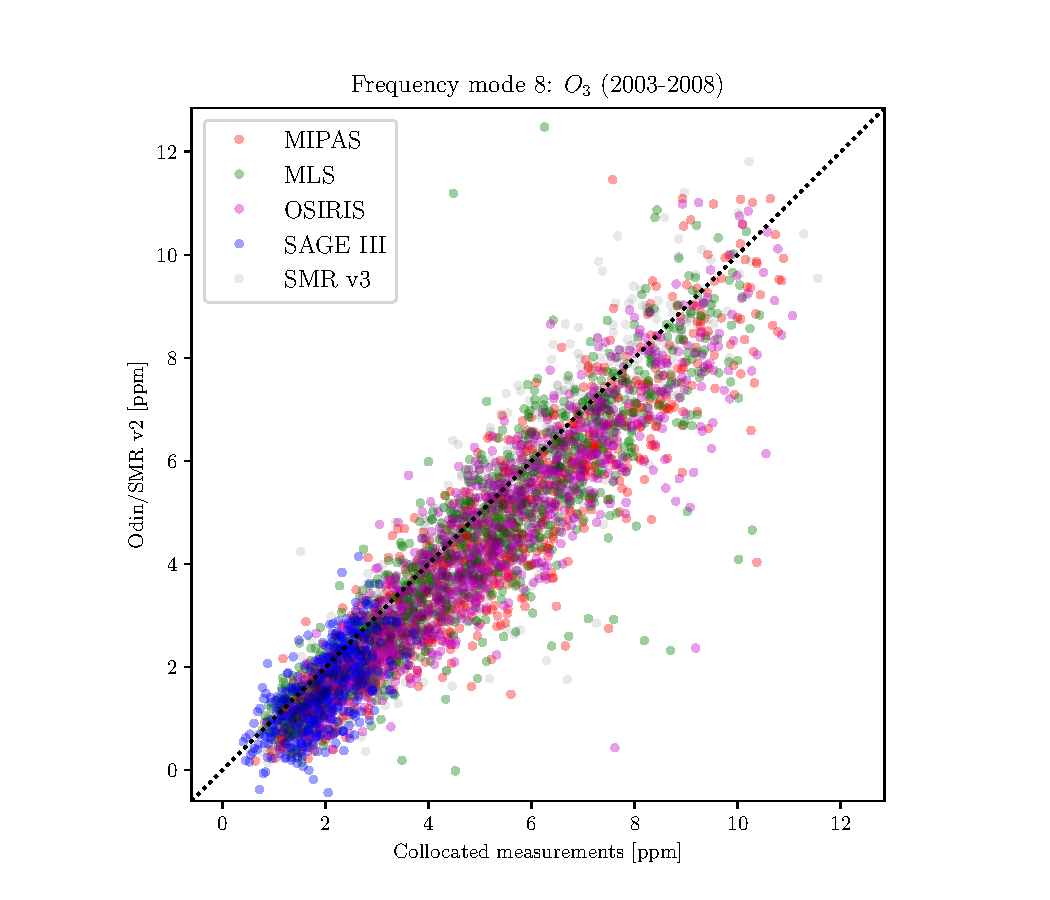
\includegraphics[width=\textwidth]{DDS_fm8_O3_scatter_v2}
        \caption{correlation of collcated instruments with \smr~v2.X}
        \label{fig:fm08:O3:scatter:v2}
    \end{subfigure}
    \,
    \begin{subfigure}[b]{0.49\textwidth}
        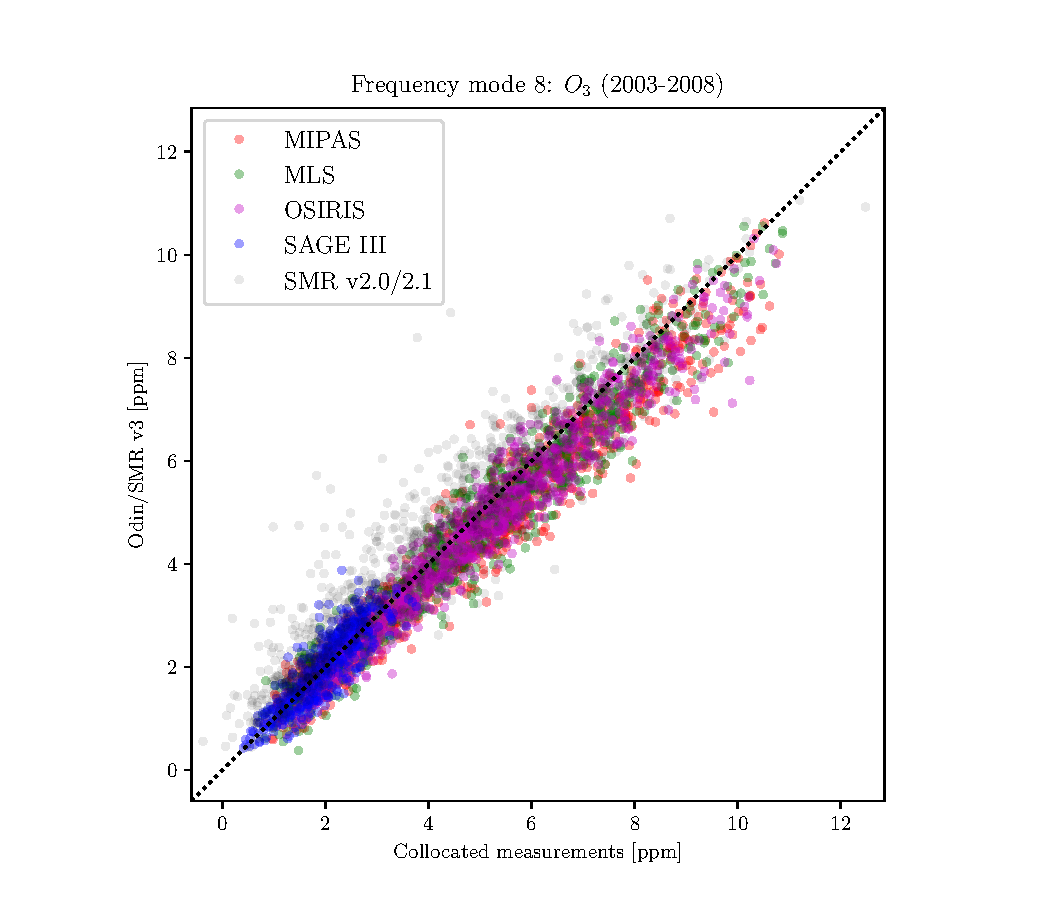
\includegraphics[width=\textwidth]{DDS_fm8_O3_scatter_v3}
        \caption{correlation of collcated instruments with \smr~v3}
        \label{fig:fm08:O3:scatter:v3}
    \end{subfigure}
    \caption{Correlation between retrievals of \chem{O_3} using \smr\
    versions~2.X and~3 and collocated measurements from various instruments
    for frequency mode~08.}
    \label{fig:fm08:O3:scatter}
\end{figure}

\begin{figure}[htpb]
    \centering
    \begin{subfigure}[b]{0.49\textwidth}
        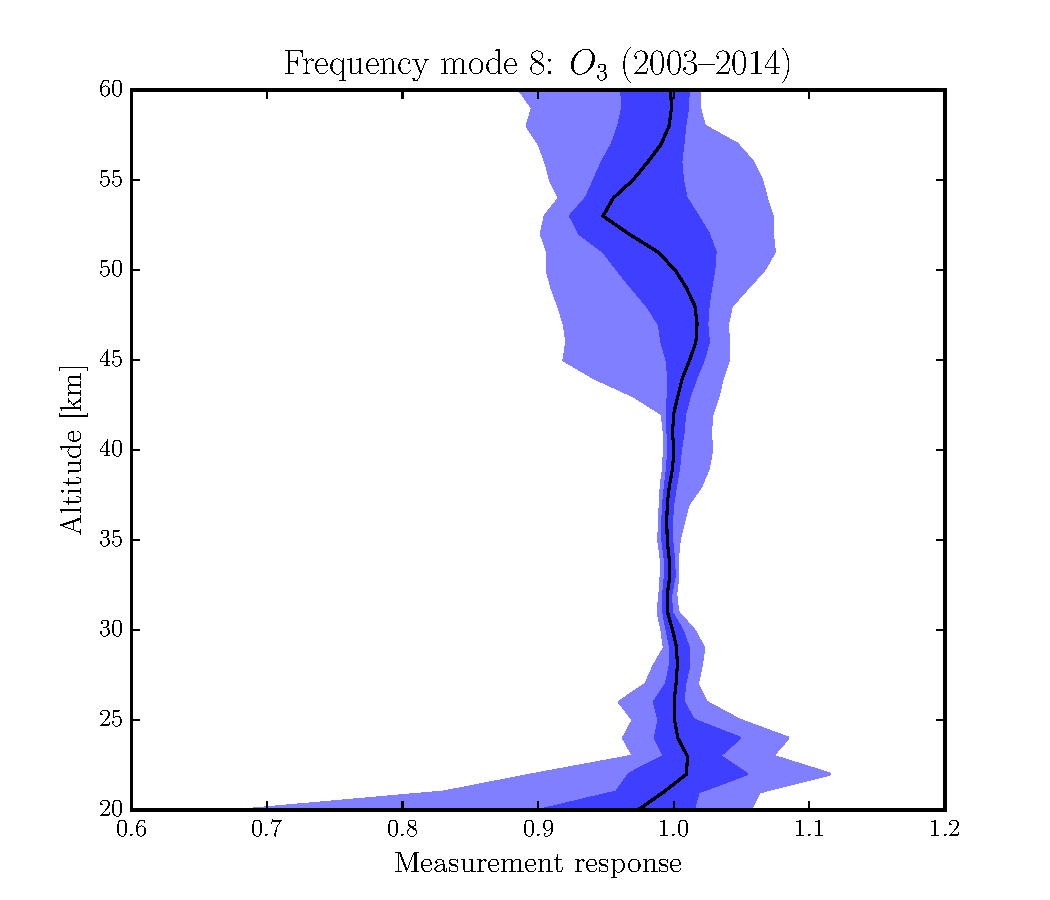
\includegraphics[width=\textwidth]{DDS_fm8_O3_mr}
        \caption{median measurement response with $1\sigma$ and $2\sigma$
        percentiles}
        \label{fig:fm08:O3:mr}
    \end{subfigure}
    \,
    \begin{subfigure}[b]{0.49\textwidth}
        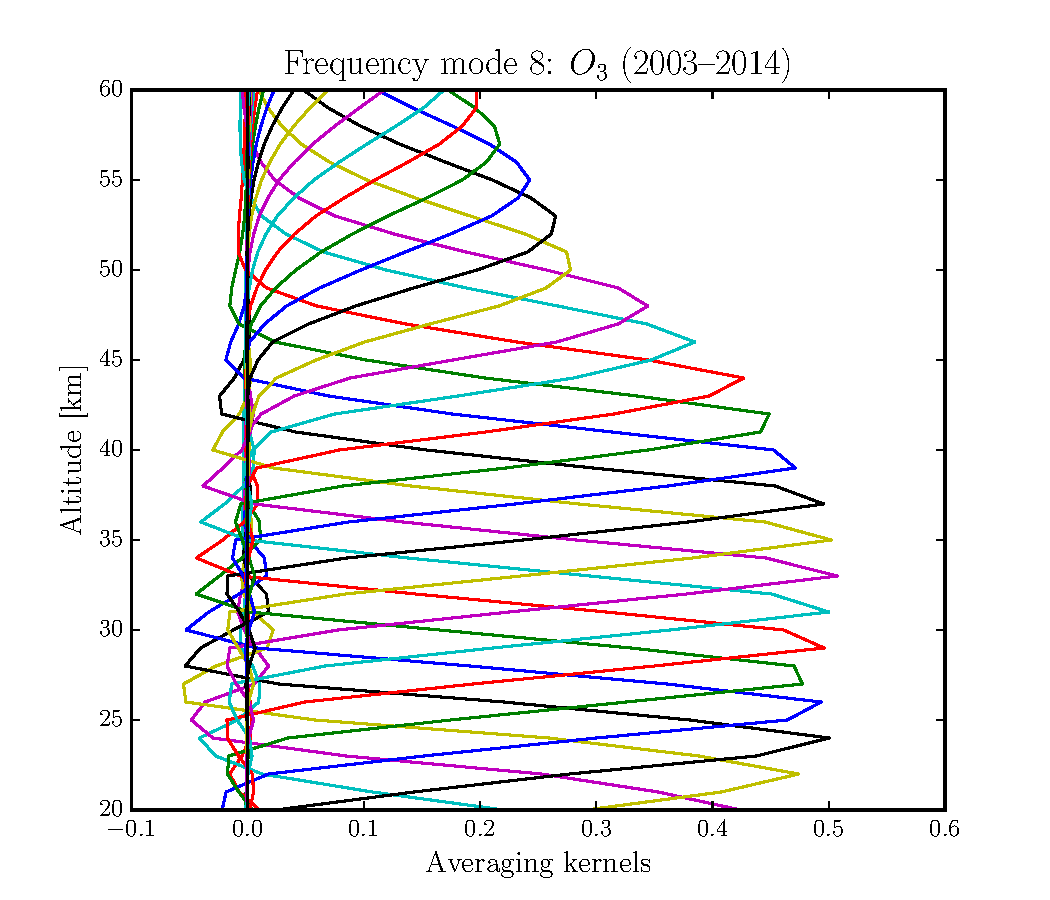
\includegraphics[width=\textwidth]{DDS_fm8_O3_avk}
        \caption{median averaging kernels\newline~}
        \label{fig:fm08:O3:avk}
    \end{subfigure}
    \caption{Measurement response and averaging kernels for \chem{O_3}
    retrievals for \smr~v3 at different altitudes for frequency mode~08.}
    \label{fig:fm08:O3:mr_avk}
\end{figure}


%%%%%%%
% H2O %
%%%%%%%

\subsubsection{\chem{H_2O}}
\label{sec:fm08:comparison:H2O}
The retrievals for \chem{H_2O} have been compared with data from the MIPAS,
MLS and SAGE~III instruments. Annual average differences to these instruments
are shown in Figure~\ref{fig:fm08:H2O:profiles}. In
Figure~\ref{fig:fm08:H2O:scatter} individual retrievals for the instruments for
the entire period are plotted against the retrievals from the new and old
versions of the \smr\ processing chain. Though the results show a considerable
improvement with the updated version of the processing compared to all
considered instruments, the correlation is still poor, and the water content is
still systematically underestimated, in particular for higher concentrations.
\TODO{reference Fig.~\ref{fig:fm08:H2O:mr_avk} in text!}

\begin{figure}[htpb]
    \centering
    \begin{subfigure}[b]{0.49\textwidth}
        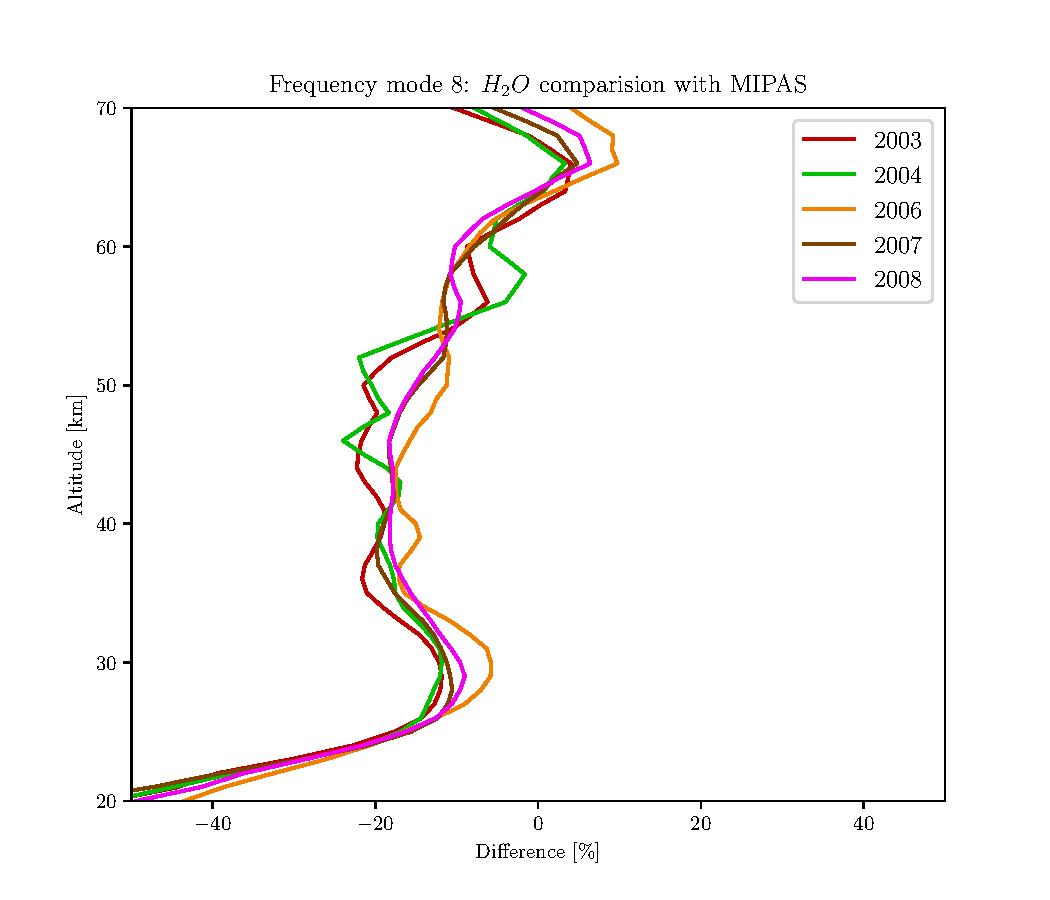
\includegraphics[width=\textwidth]{DDS_fm8_H2O_perdiff_mipas}
        \caption{average difference to MIPAS}
        \label{fig:fm08:H2O:profiles:MIPAS}
    \end{subfigure}
    \,
    \begin{subfigure}[b]{0.49\textwidth}
        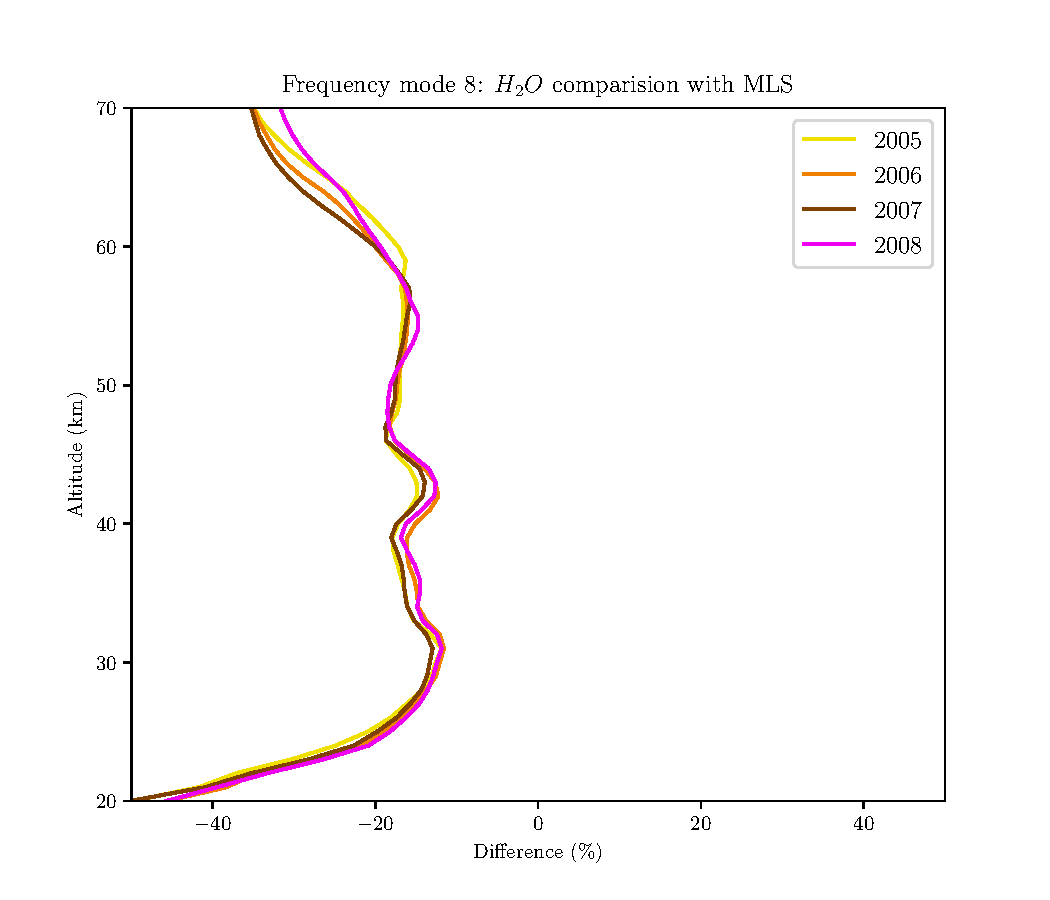
\includegraphics[width=\textwidth]{DDS_fm8_H2O_perdiff_mls}
        \caption{average difference to MLS}
        \label{fig:fm08:H2O:profiles:MLS}
    \end{subfigure}

    \begin{subfigure}[b]{0.49\textwidth}
        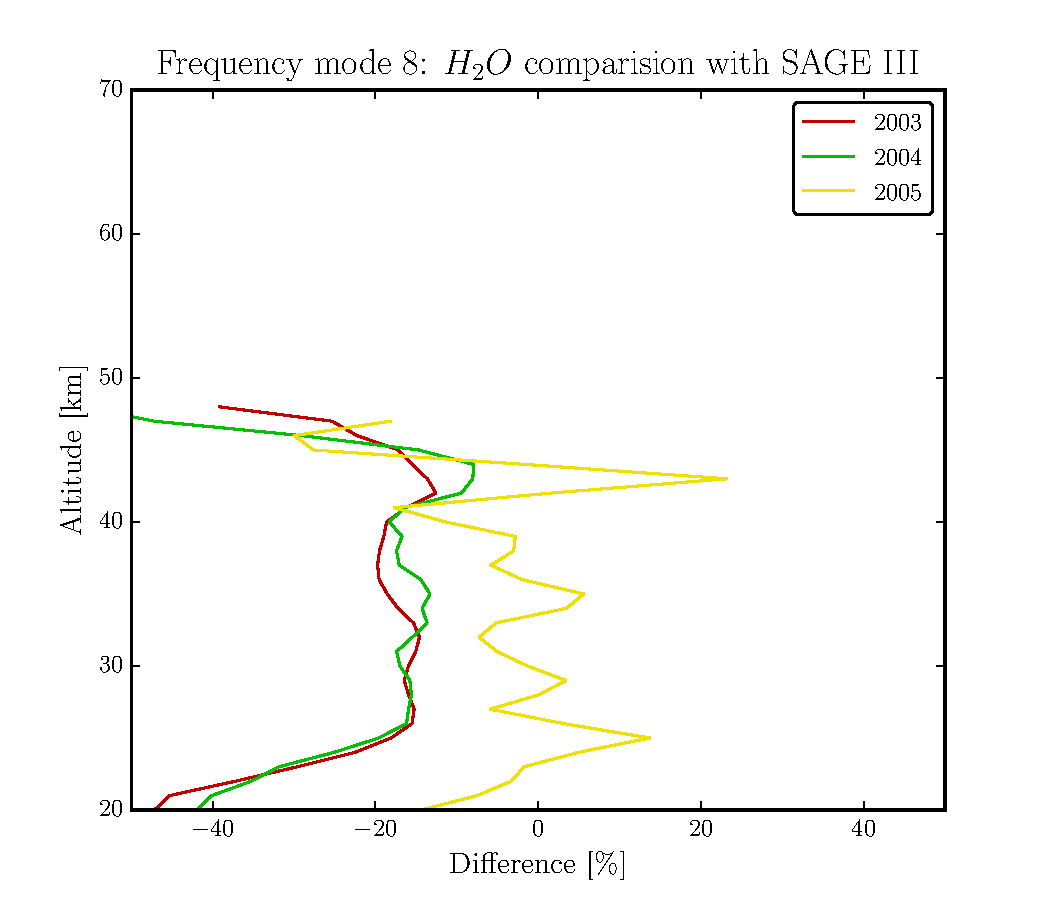
\includegraphics[width=\textwidth]{DDS_fm8_H2O_perdiff_sage}
        \caption{average difference to SAGE~III}
        \label{fig:fm08:H2O:profiles:SAGEIII}
    \end{subfigure}
    \caption{Average difference in percent between retrievals of \chem{H_2O}
    from \smr~v3 and collocated measurements from various instruments at
    different altitudes for frequency mode~08.}

    \label{fig:fm08:H2O:profiles}
\end{figure}

\begin{figure}[htpb]
    \centering
    \begin{subfigure}[b]{0.49\textwidth}
        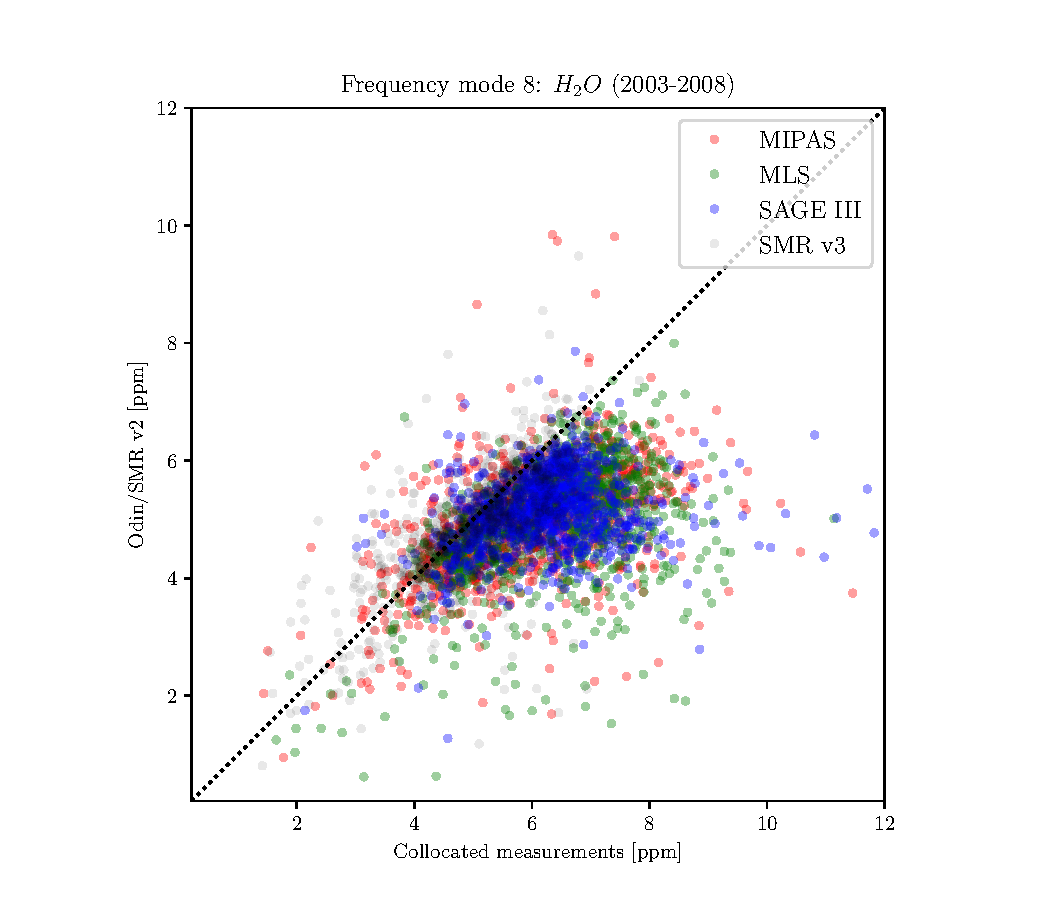
\includegraphics[width=\textwidth]{DDS_fm8_H2O_scatter_v2}
        \caption{correlation of collcated instruments with \smr~v2.X}
        \label{fig:fm08:H2O:scatter:v2}
    \end{subfigure}
    \,
    \begin{subfigure}[b]{0.49\textwidth}
        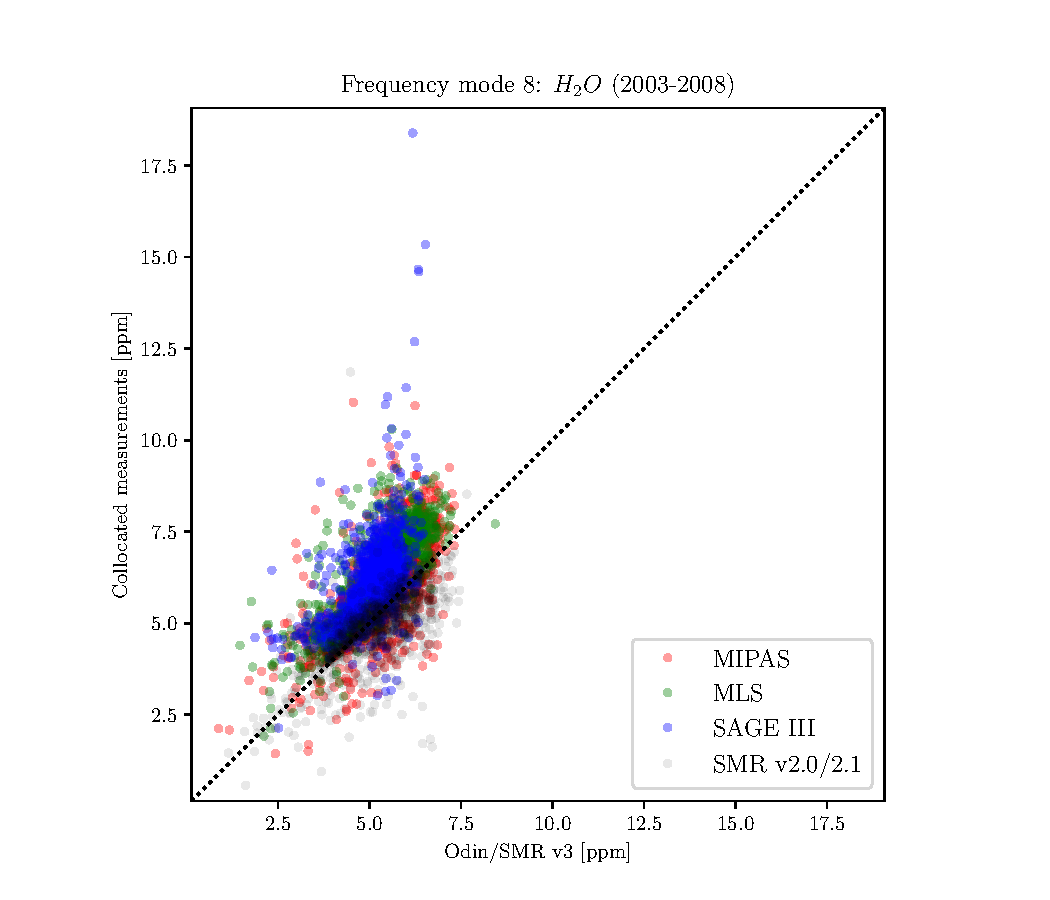
\includegraphics[width=\textwidth]{DDS_fm8_H2O_scatter_v3}
        \caption{correlation of collcated instruments with \smr~v3}
        \label{fig:fm08:H2O:scatter:v3}
    \end{subfigure}
    \caption{Correlation between retrievals of \chem{H_2O} using \smr\
    versions~2.X and~3 and collocated measurements from various instruments
    for frequency mode~08.}
    \label{fig:fm08:H2O:scatter}
\end{figure}

\begin{figure}[htpb]
    \centering
    \begin{subfigure}[b]{0.49\textwidth}
        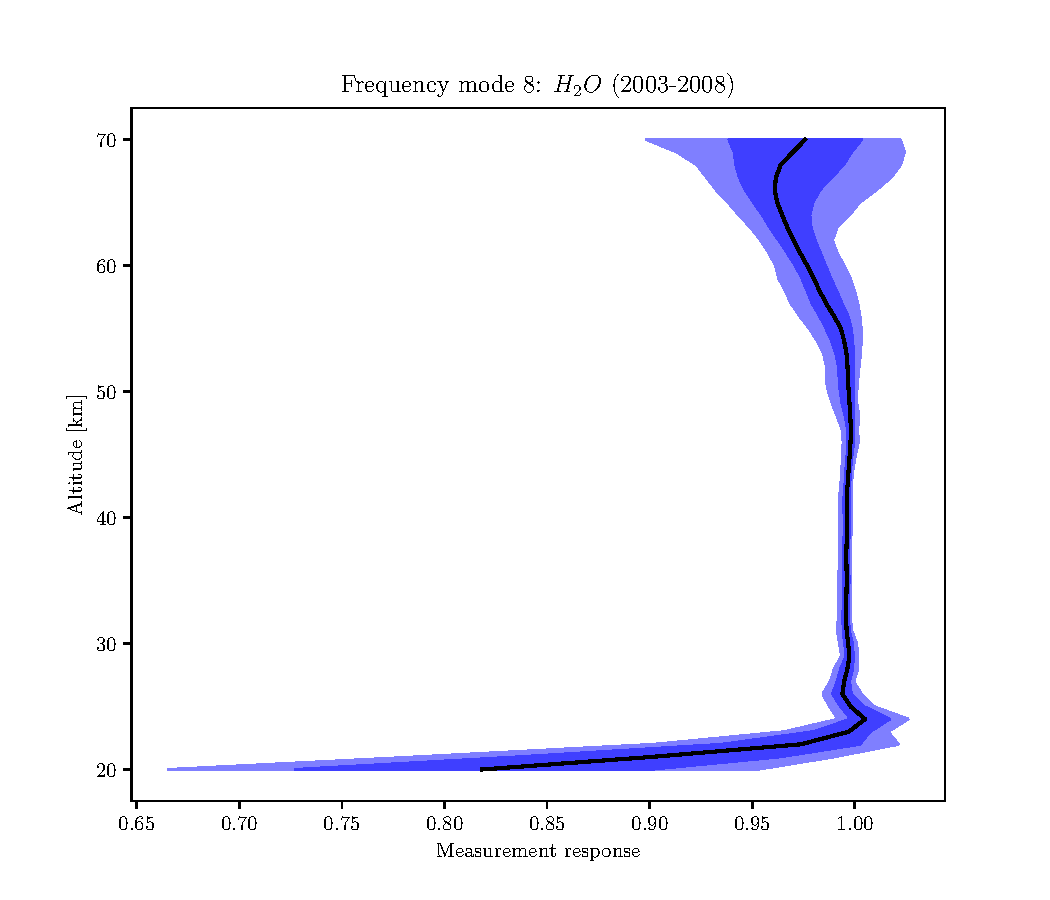
\includegraphics[width=\textwidth]{DDS_fm8_H2O_mr}
        \caption{median measurement response with $1\sigma$ and $2\sigma$
        percentiles}
        \label{fig:fm08:H2O:mr}
    \end{subfigure}
    \,
    \begin{subfigure}[b]{0.49\textwidth}
        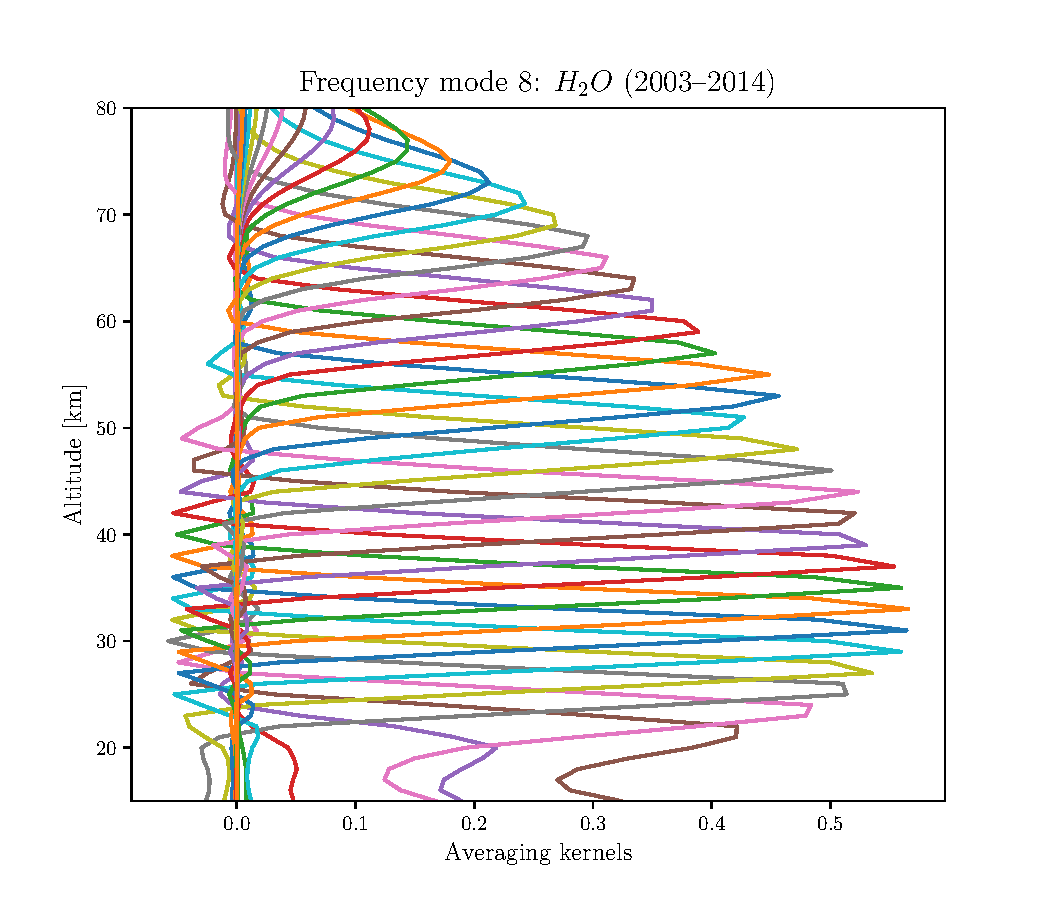
\includegraphics[width=\textwidth]{DDS_fm8_H2O_avk}
        \caption{median averaging kernels\newline~}
        \label{fig:fm08:H2O:avk}
    \end{subfigure}
    \caption{Measurement response and averaging kernels for \chem{H_2O}
    retrievals for \smr~v3 at different altitudes for frequency mode~08.}
    \label{fig:fm08:H2O:mr_avk}
\end{figure}


\subsection{Discussion}
\label{sec:fm08:discussion}
The Pearson correlation between the \smr\ retrievals and the other instruments
was calculated for the entire period for both versions of the processing chain.
The results are summarised in Table~\ref{tab:fm08:stats}, and show that the
new algorithm is a improvement compared to all the instruments for all species
used in this investigation. The improvement is considerable for both \chem{O_3}
and \chem{H_2O}.


\begin{table}[hbt]
\centering
\caption{Pearson correlation and fit parameters of the old and new \smr\
retrievals for frequency mode~08, compared with collocated data from other
instruments for the period 2003--2008.
}
\label{tab:fm08:stats}
\begin{tabular}{lllrrrr}
    \toprule
    \textbf{Species} & \textbf{Instrument} & \textbf{SMR} & \textbf{corr.} & \textbf{slope} & \textbf{intercept} & \textbf{$\left|\left<\right.\right.$res.$\left.\left.\right>\right|$} \\
    \midrule
    \chem{O3}   & MIPAS     & v3    & 0.978 & 0.905 & 0.073\,ppm    & 0.632\,ppm \\
                &           & v2.x  & 0.930 & 0.910 & -0.346\,ppm   & 1.206\,ppm \\
    \cline{2-7}
                & MLS       & v3    & 0.980 & 0.925 & 0.108\,ppm    & 0.530\,ppm \\
                &           & v2.x  & 0.911 & 0.921 & -0.223\,ppm   & 1.144\,ppm \\
    \cline{2-7}
                & OSIRIS    & v3    & 0.975 & 0.927 & 0.045\,ppm    & 0.560\,ppm \\
                &           & v2.x  & 0.917 & 0.931 & -0.311\,ppm   & 1.095\,ppm \\
    \cline{2-7}
                & SAGE III  & v3    & 0.884 & 0.956 & 0.134\,ppm    & 0.357\,ppm \\
                &           & v2.x  & 0.658 & 0.804 & -0.026\,ppm   & 0.752\,ppm \\
    \midrule
    \chem{H_2O} & MIPAS     & v3    & 0.702 & 0.565 & 1.807\,ppm    & 1.261\,ppm \\
                &           & v2.x  & 0.480 & 0.344 & 2.852\,ppm    & 1.637\,ppm \\
    \cline{2-7}
                & MLS       & v3    & 0.801 & 0.684 & 0.867\,ppm    & 1.342\,ppm \\
                &           & v2.x  & 0.419 & 0.369 & 2.683\,ppm    & 1.799\,ppm \\
    \cline{2-7}
                & SAGE III  & v3    & 0.528 & 0.317 & 3.061\,ppm    & 1.657\,ppm \\
                &           & v2.x  & 0.241 & 0.128 & 4.353\,ppm    & 0.925\,ppm \\
    \bottomrule
\end{tabular}
\end{table}

\subsection{Conclusions}
\label{sec:fm08:conclusions}
\TODO{Recommended usage: which species, which periods}
Based on the discussion above, retrievals based on frequency mode~08 can be
used with confidence for the species \chem{O_3} but should be used with some
caution for \chem{H_2O}.
